\documentclass[12pt,oneside]{scrreprt}
\usepackage[T1]{fontenc}		% Einstellungen fuer Umlaute usw.
\usepackage[utf8x]{inputenc}
\usepackage[ngerman]{babel}
\usepackage{listings}
\usepackage{float}
\usepackage{fancyvrb}
\usepackage{parskip}
\usepackage{setspace}
\usepackage[official]{eurosym}			% Einstellungen fuer Absaetze: Abstand statt Einrueckung
\addtokomafont{disposition}{\rmfamily}

\usepackage[a4paper,			% Papierformat A4
	    left=2.5cm,				% linker Rand
	    right=2.5cm,			% rechter Rand
	    top=1.5cm,				% oberer Rand 
	    bottom=1.5cm,			% unter Rand
	    marginparsep=5mm,		% Abstand der Randnotizen
	    marginparwidth=10mm, 	% Breite der Randnotizen
	    headheight=7mm,			% Hoehe der Kopfzeile
	    headsep=1.2cm,			% Abstand der Kopfzeile
	    footskip=1.5cm,			% Abstand der Fusszeile
	    includeheadfoot]{geometry}

\usepackage{fancyhdr}						% Konfiguration von Kopf- und Fusszeilen
\pagestyle{fancy}							% Seitenstil 'fancy'
\fancyhf{}									% vorhandene Einstellungen loeschen
\setlength{\headwidth}{\textwidth}			% Kopf- und Fusszeile so breit wie der Haupttext
\fancyfoot[R]{\thepage} 					% Festlegung des Seitenstils: Seitenzahlen in der Fusszeile rechts
\fancyfoot[L]{\leftmark}					% Kapitelnr. und -Bezeichnung in der Fusszeile links
\fancyhead[R]{\IhreArbeit}					% "Bachelorarbeit" in der Kopfzeile rechts
\fancyhead[L]{\IhrVorname\ \IhrNachname}	% Vorname und Name in der Kopfzeile links
\renewcommand{\chaptermark}[1]{			% Definition der Ausgabe des Kapitels
  \markboth{Kapitel \thechapter. #1}{}}
\renewcommand{\headrulewidth}{0.5pt}		% Trennlinie zwischen Kopfzeile und Haupttext
\renewcommand{\footrulewidth}{0.5pt}		% Trennlinie zwischen Haupttext und Fusszeile
\fancypagestyle{plain}{					% Anpassung des Seitenstils 'plain' bei Beginn neuer Kapitel
  \fancyhf{}								% Vorbelegung loeschen
  \fancyfoot[C]{\thepage}					% Seitenzeilen in der Fusszeile mittig
  \fancyhead[R]{\IhreArbeit}				% "Bachelorarbeit" in der Kopfzeile rechts
  \fancyhead[L]{\IhrVorname\ \IhrNachname}	% Vorname und Name in der Kopfzeile links
}

\usepackage{amsmath}			% Pakete fuer den Mathematikmodus
\usepackage{amssymb}
\usepackage[intlimits]{empheq}

\usepackage[sc]{mathpazo}		% Schriftart Palatino fuer Haupttext und Mathematikmodus
\usepackage{pifont}				% zusaetzliche Symbole
\usepackage{csquotes}

\usepackage[format=hang,		% Einstellung fuer Bildunterschriften
            font={footnotesize},
            labelfont={bf},
            margin=1cm,
            aboveskip=5pt,
            position=bottom]{caption}

\usepackage{graphicx}							% Einbinden von Graphiken
\usepackage[svgnames,table,hyperref]{xcolor} 	% Verwendung von Farben
\usepackage{tikz}								% Erstellen von Grafiken
\usetikzlibrary{positioning,arrows,plotmarks} % TikZ-Bibliotheken
%\usepackage{pgfplots}                           % Darstellung von Plots, Funktionen, Graphen usw.

%
% Weitere Pakete
%
%\usepackage{listings}			% Darstellung von Quellcode
%\lstset{language=Python, basicstyle=\ttfamily, numbers=none}
%
%\usepackage[european, siunitx]{circuitikz}	% Darstellung von Schaltungen
%
%\usepackage{enumerate}			% Formatierung nummerierter Listen

\usepackage{microtype,relsize}					% Wird verwendet, um Nachnamen auf Titelseite gesperrt darzustellen
\newcommand*{\Sperren}[1]{\textls*[100]{#1}}

% 
% Persoenliche Angaben
% 
% 
\newcommand*{\IhrVorname}{Daniel}
\newcommand*{\IhrNachname}{Schneider}
\newcommand*{\IhrStudiengang}{Internationaler Studiengang Medieninformatik}
\newcommand*{\IhreArbeit}{Masterarbeit}
\newcommand*{\IhrTitelDE}{Photogrammetrie zur Platzierung von standortbezogenen dynamischen Inhalten in AR}
\newcommand*{\IhrTitelEN}{Photogrammetry for placement of location-based dynamic content in AR}
\newcommand*{\IhrBearbeitungszeitraumVON}{13.05.2019}
\newcommand*{\IhrBearbeitungszeitraumBIS}{16.09.2019}
\newcommand*{\IhrErstpruefer}{Prof. Dr. Tobias Lenz}
\newcommand*{\IhrZweitpruefer}{Prof. Dr. Klaus Jung}
\newcommand*{\IhreFirma}{HTW Berlin}
\newcommand*{\IhrFirmenbetreuer}{}
\newcommand*{\IhreZusammenfassung}{ Diese Arbeit analysiert die wichtigsten Verfahren aus der Photogrammetrie und der Computer Vision, wie den Bündelblockausgleich, SLAM (Simultaneous Location and Mapping) und SfM (Structure from Motion) im Kontext von Augmented Reality (AR) für Android Smartphones. Die Algorithmen der beiden Disziplinen werden in Zusammenhang gestellt und eine inhaltliche Unterscheidung, trotz der Überschneidung der Algorithmen, formuliert. Die Tauglichkeit der photogrammetrischen Verfahren wird in Bezug zu Augmented Reality geprüft. Im Praxisteil dieser Arbeit wird eine Anwendung erstellt, die ein aktuelles AR Framework verwendet, welches SLAM implementiert. }
\newcommand*{\IhreSchluesselwoerter}{Photogrammetrie, Computer Vision (CV), Augmented Reality (AR), standortbezogene Daten, Android, Java, Structure from Motion (SfM), Simultaneous Location and Mapping (SLAM)}


\usepackage[bookmarks, raiselinks, pageanchor, % PDF-Einstellungen
            hyperindex, colorlinks,
            citecolor=black, linkcolor=black,
            urlcolor=black, filecolor=black,
            menucolor=black]{hyperref}
\hypersetup{pdftitle={\IhrTitelDE},%
            pdfauthor={\IhrVorname\ \IhrNachname},%
            pdfsubject={\IhreArbeit},%
            pdfkeywords={\IhreSchluesselwoerter}}


%
% Beginn des Textteils
%
\begin{document}
  \pagenumbering{roman}
  \begin{titlepage}					% Titelseite
    \thispagestyle{empty}
    \begin{center}
      \Large
      Hochschule für Technik und Wirtschaft Berlin\\[1cm]
      \IhrStudiengang\\[1cm]
      \textbf{\IhreArbeit}\\[1cm]
      von\\[1cm]
      \IhrVorname\ \Sperren{\textbf{\IhrNachname}}\\[1cm]
      \textbf{\IhrTitelDE}\\[1cm]
      \IhrTitelEN
    \end{center}
  \end{titlepage}
  \clearpage
  \thispagestyle{empty}			% 1. Seite soll eine Leerseite sein (dazu muss ein Trick verwendet werden)
  \mbox{}
  \clearpage
  \thispagestyle{empty}			% 2. Seite wie Titelseite, aber mit zusaetzlichen Angaben
  \begin{center}
    \Large
    Hochschule für Technik und Wirtschaft Berlin\\
    Fachbereich Informatik, Kommunikation und Wirtschaft\\[1cm]
    Studiengang \IhrStudiengang\\[1cm]
    \textbf{\IhreArbeit}\\[1cm]
    von\\[1cm]
    \IhrVorname\ \Sperren{\textbf{\IhrNachname}}\\[1cm]
    \textbf{\IhrTitelDE}\\[1cm]
    \IhrTitelEN
  \end{center}
  \vspace*{5cm}
  \begin{tabbing}
    \underbar{Bearbeitungszeitraum:}\qquad\= von\qquad\=\IhrBearbeitungszeitraumVON\\
                                          \> bis      \>\IhrBearbeitungszeitraumBIS
  \end{tabbing}
  \vspace*{1cm}
  \underbar{1. Prüfer:}\qquad\IhrErstpruefer\par 
  \underbar{2. Prüfer:}\qquad\IhrZweitpruefer
  \clearpage
  % formblatt_para12apo.tex
%

\thispagestyle{empty}				% Formblatt Bestaetigung nach Paragraph 12 APO
\begin{minipage}{0.65\textwidth}
  Hochschule für Technik und Wirtschaft Berlin\\
  Fachbereich Informatik, Kommunikation und Wirtschaft\\[1.5cm]
\end{minipage}

Eigenständigkeitserklärung\\
\rule[1ex]{\textwidth}{0.5pt}
\vspace*{0.5cm}
\begin{tabbing}
  Name und Vorname\\
  der Studentin/des Studenten:\qquad\=\textbf{\IhrNachname, \IhrVorname}\\[1cm]
  Studiengang:                      \>\textbf{\IhrStudiengang}
\end{tabbing}
\rule[1ex]{\textwidth}{0.5pt}
\vspace*{0.5cm}
Ich bestätige, dass ich die \IhreArbeit\ mit dem Titel:
\begin{center}
  \textbf{\IhrTitelDE}
\end{center}
\vspace*{0.5cm}
selbständig verfasst, noch nicht anderweitig für Prüfungszwecke vorgelegt, keine anderen als die angegebenen Quellen oder Hilfsmittel benutzt sowie wörtliche und sinngemäße Zitate als solche gekennzeichnet habe.\\[0.5cm]
\rule[1ex]{\textwidth}{0.5pt}
\begin{tabbing}
  Datum:\hspace{2cm}\=\today\\[1cm]
  Unterschrift:\> 
\end{tabbing}
\rule[1ex]{\textwidth}{0.5pt}
\clearpage		% 3. Seite: Formblatt Bestaetigung nach Paragraph 12 APO
  % formblatt_summary.tex
%

\thispagestyle{empty}				% Formblatt Zusammenfassung
\begin{minipage}{0.65\textwidth}
  Hochschule für Technik und Wirtschaft Berlin\\
  Fachbereich Informatik, Kommunikation und Wirtschaft\\[1.5cm]
\end{minipage}

\IhreArbeit\ Zusammenfassung\\
\rule[1ex]{\textwidth}{0.5pt}
\vspace*{0.5cm}
\begin{tabular}{lp{6.5cm}}
  \hspace*{-1ex}Studentin/Student (Name, Vorname): & \textbf{\IhrNachname, \IhrVorname}\\
  \hspace*{-1ex}Studiengang: & \IhrStudiengang\\
  \hspace*{-1ex}Aufgabensteller, Professor: & \IhrErstpruefer\\
  \hspace*{-1ex}Durchgeführt in (Firma/Behörde/Hochschule): & \IhreFirma\\
  \hspace*{-1ex}Betreuer in Firma/Behörde: & \IhrFirmenbetreuer\\
  \multicolumn{2}{l}{\hspace*{-1ex}Ausgabedatum: \IhrBearbeitungszeitraumVON\qquad\qquad Abgabedatum: \IhrBearbeitungszeitraumBIS}
\end{tabular}\par 
\rule[1ex]{\textwidth}{0.5pt}
Titel:
\begin{center}
  \textbf{\IhrTitelDE}
\end{center}
\vspace*{0.5cm}
\rule[1ex]{\textwidth}{0.5pt}
Zusammenfassung:\\[0.5cm]
\IhreZusammenfassung\\[0.5cm]
Schlüsselwörter: \IhreSchluesselwoerter
\clearpage			% 4. Seite: Formblatt Zusammenfassung
  \tableofcontents
  \newpage
  \pagenumbering{arabic}
  \onehalfspacing
  \chapter{Motivation}

Photogrammetrie ist \glqq die Wissenschaft und Technologie der Gewinnung von Informationen
über die physische Umwelt aus Bildern, mit einem Schwerpunkt auf Vermessung,
Kartierung und hochgenauer Messtechnik\grqq{} (Heipke, 2017, S.5 \cite{photo}).  Die Photogrammetrie beschäftigt sich  mit der Rekonstruktion von dreidimensionalen Daten aus zweidimensionalen Informationsträgern, wie Bildern oder Laserscandaten. Dabei gehen diese Daten alle auf das Prinzip der Aufnahme der elektromagnetischen Strahlung zurück. Bei Bildern ist das die Helligkeits- und Farbverteilung, bei Laserscans sind es Entfernungsbilder, beziehungsweise Punktwolken. Die Disziplin der Photogrammetrie ist dabei dem Bereich der Fernerkundung zuzuordnen, die sich mit der Auswertung von geometrischen oder semantischen Informationen beschäftigt. Beides sind Fachbereiche, die sich über die Jahrzehnte entwickelt haben und sich dem Gebiet der Geodäsie zuordnen lassen. Die Geodäsie erfasst Geoinformationen über die Erde, die dann beispielsweise mit Kartographie visualisiert werden können. Das große Potenzial der Bereitstellung und Gewinnung von dreidimensionalen Daten war in der Photogrammetrie seit Beginn eine der wichtigsten Stärken der Technologie. Photogrammetrie wird von Raumsonden im All bis hin zur Mikroskopie eingesetzt. Auch wenn die ursprüngliche Kernanwendung die Kartenerstellung war, sind nicht-topographische Anwendungen seit der Einführung digitaler Kameras stark expandiert. Dazu zählt zum Beispiel die hochpräzise industrielle Messtechnik, die architektonische Photogrammetrie, die medizinische und forensische Bildgebung und Analyse, sowie die Erstellung von dreidimensionalen Modellen aus Fotoserien oder Laserdaten, welche der Nahbereichsphotogrammetrie zugeordnet werden kann (vgl. \cite{state_of_art} S.1).


Das Gebiet der Computer Vision (CV), das sich in den letzten Jahren teilweise parallel mit der Photogrammetrie entwickelt hat, verfolgt einen ähnlichen Ansatz und ist deshalb inhaltlich mit der digitalen Photogrammetrie verwandt. In diesem Bereich haben sich ebenfalls verschiedene Verfahren zur Kartierung der Umwelt und der gleichzeitigen Lokalisierung in dieser entwickelt, welche ebenfalls in dieser Arbeit beschrieben werden.  \\ \\

Das Forschungsziel der Computer Vision ist es, anhand von zweidimensionalen Bildern oder Videos die geometrischen Informationen von dreidimensionalen Objekten, wie Form, Position, räumlicher Lage, Bewegung oder Daten über den Inhalt der Bilder zu gewinnen, sowie dem Computer ein umfassenes \glqq Verständnis\grqq{} der Inhalte der Bilder zu ermöglichen (vgl. \cite{photo} S. 5-7).

Durch die Entwicklung der Technik der letzten Jahrzehnte und der damit eingehenden Steigerung der Rechenpower bei mobilen Endgeräten haben sich die Bereiche vergrößert, in denen digitale Photogrammetrie, sowie Verfahren aus der CV eingesetzt werden können. Im Rahmen dieser Arbeit soll evaluiert werden, ob photogrammetrische Verfahren für Augmented Reality Anwendungen im Bereich von Smarthphones eingesetzt werden können, um in Echtzeit aus Videodaten die dreidimensionale Beschaffenheit der gefilmten Objekte zu rekonstruieren. Dazu werden, nach einer kurzen Definition und Einführung in Augmented Reality, die Verfahren und Algorithmen aus der Photogrammetrie und der Computer Vision analysiert und verglichen. Es werden weiterhin Vorteile sowie Nachteile der jeweiligen Disziplinen aufgezeigt und anschließend im Kontext zu Augmented Reality beschrieben. 

Im Rahmen dieser Arbeit ist weiterhin eine auf dem Android Betriebsystem basierende Anwendung erstellt worden, welche eine der neuen Technologien im Bereich Augmented Reality implementiert und aktuelle Frameworks und Bibliotheken verwendet. Die Besonderheiten dieser Frameworks werden im Praxisteil dieser Arbeit beschrieben.



  



  \chapter{Augmented Reality}

Im Gegensatz zu \glqq Virtual Reality\grqq{} (VR), welche eine interaktive, dreidimensionale, computergenerierte, immersive Umgebung schafft, in die eine Person versetzt wird, erlaubt \glqq Augmented Reality\grqq{} (AR) die Überblendung von digitalen Medieninformationen über die Wahrnehmung der echten Welt. Dadurch fällt AR in die Definition von \glqq Mixed Reality\grqq{} (MR).

\begin{figure}[H]
	\centering
	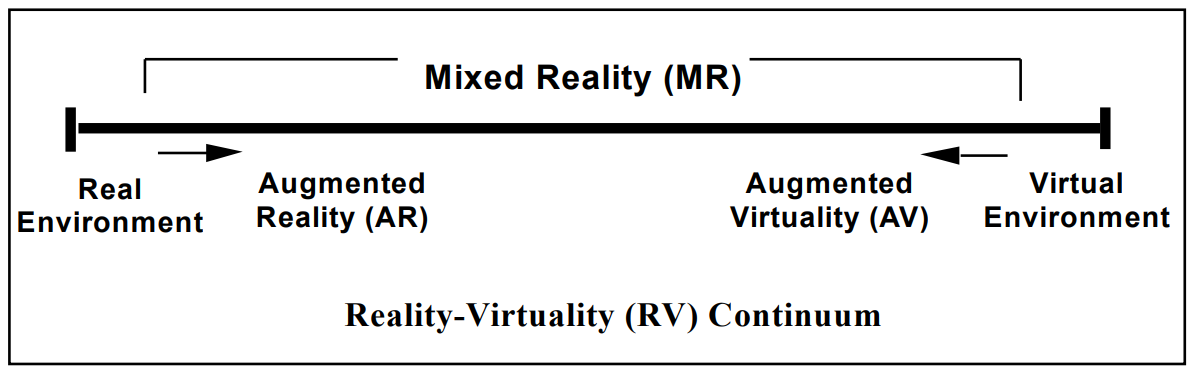
\includegraphics[scale=0.52]{ar_vr.png}
	\caption{Das Realität - Virtualität Kontinuum, Bildquelle \cite{ar_vr}}
\end{figure} 

Im Rahmen dieser Arbeit wird sich, wenn der Begriff Augmented Reality (AR) verwendet wird, auf Monitor basierte, nicht immersive Geräte bezogen, da sich in der Analyse der Verfahren und der Implementation einer AR Anwendung, auf Smartphones bezogen wird. Diese Anzeigesysteme werden auch als \glqq window-on-the-world\grqq{} bezeichnet, da computergenerierte Bilder oder Informationen digital über das Echtzeit Kamera Bild überlagert werden. (vgl. \cite{ar_vr} S.284)



\section{Augmented Reality - Software Development Kits}

\glqq Software Development Kits\grqq (SDK) oder auch Frameworks, sind Werkzeuge und Bibliotheken, welche eine Programmierumgebung und Basistechnologien liefern, um Programme zu entwickeln. Im Bereich von Augmented Reality umfassen Frameworks meistens die drei Hauptkomponenten: (vgl. \cite{sdks} S.3)

\begin{itemize}

\item \textbf{Recognition}: Erkennung von Bildern, Objekten, Gesichtern oder Räumen, auf welche die virtuellen Objekte oder Informationen überlagert werden können.


\item \textbf{Tracking}: Echtzeit-Lokalisierung der erkannten Objekte und Berechnung der lokalen Position des Gerätes zu diesen.

\item \textbf{Rendering}: Überlagerung der virtuellen Medieninformationen über das Bild und Anzeige der generieren Mixed Reality.
\end{itemize}

\subsection{Marktübersicht - Software Development Kits}

Die folgende Tabelle gibt eine Übersicht an gängigen SDKs, und deren Plattformkompatibilität. \\

\begin{table}[h!]
\hskip-1.5cm
\begin{tabular}{|l|l|l|l|l|l|l|l|l|l|}
\hline
        & Vuforia & Wikitude & Metaio & ARToolKit & Kudan & EasyAR & MaxST & ARCore & ARKit \\ \hline
Android &   \checkmark      &    \checkmark      &    \checkmark    &     \checkmark      &   \checkmark    &    \checkmark    &    \checkmark   &     \checkmark   &    x   \\ \hline
iOS     &    \checkmark      &   \checkmark        &   \checkmark      &    \checkmark        &   \checkmark    &    \checkmark     &   \checkmark     &    \checkmark     &    \checkmark    \\ \hline
Windows &     \checkmark     &    \checkmark       &     \checkmark    &    \checkmark        &   x    &     \checkmark    &  \checkmark      &    x    &    x   \\ \hline
\end{tabular}
\end{table}


Bis auf das von Apple entwickelte ARKit, sind alle hier genannten Frameworks für Android verwendbar. Weiterhin unterstützen alle das Betriebsystem iOS, sowie Windows, bis auf Kudan, ARCore und ARKit. Im praktischen Teil dieser Arbeit werden mehrere dieser Software Development Kits auf der Android Plattform verwendet, getestet und analysiert.

\section{Voraussetzungen für Augmented Reality}
Augmented Reality Anwendungen haben hohe Anforderungen an die Rechnenpower der Technik, die Verarbeitungsgeschwindigkeit der Algorithmen und Robustheit der verwendeten Verfahren. (vgl. \cite{vorraussetzungen} S.1)


\begin{itemize}

\item \textbf{Hohe räumliche Genauigkeit}: 6 \glqq Degrees of Freedom\grqq{} (Freiheitsgrade) in Position und Ausrichtung. 

\item \textbf{Sehr geringer Jitter (Zittern)}: Das Rauschen im Tracking System muss minimal gehalten werden.

\item \textbf{Hohe Aktualisierungsraten}: mindestens 30Hz, besser mehrere 100Hz.

\item \textbf{Sehr geringer Lag}: Die Verzögerung von Messung bis zur Trackerausgabe muss minimal sein.

\item \textbf{Volle Mobilität}: Bewegungsfreiheit für den Nutzer: Keine Kabel, kein eingeschränkte Umfang an Bedienmöglichkeiten.
\end{itemize}

Erst durch die Entwicklung der Technik in den letzten zwei Jahrzehnten und einer damit eingehenden Steigerung der Rechenpower von mobilen Geräten hat sich Augmented Reality auf Smartphones durchsetzen können.

\section{Arten des Augmented Reality Trackings}

Das Erkennen der Umgebung und die Lokalisierung der Kamera (Camera Pose Estimation), ist der ausschlaggebende Schritt zur Realisierung von Augmented Reality. Erst dies erlaubt die Projektion von digitalen Modellen in der richtigen Position auf den echten Bildern. Präzise und robuste Kamerapositionsdaten sind eine Grundvoraussetzung für eine Vielzahl an Anwendungen, wie dynamischer Szenenanalyse und Interpretation, 3D-Szenestrukturerkennung und Videodatenkompression. Augmented Reality Umgebungen sind ein Hauptanwendungsgebiet der Kameralokalisierung, da ein eingeschränkter Arbeitsbereich hohe Anforderungen an die Robustheit und Schnelligkeit stellt. Es existieren viele verschiedene Ansätze um die Kameralokalisierung im Raum zu lösen. Das Problem wird als nichtlineares Problem betrachtet und wird meistens durch die \glqq Method of least squares\grqq{} (Methode der kleinsten Quadrate) oder nichtlineare Optimierungsalgorithmen gelöst, typischerweise durch das Gauß-Newton oder Levenberg-Marquardt Verfahren. (vgl. \cite{camera_pose} S.1) Im Folgenden werden die vier gängigsten Ansätze zur Lösung dieses Tracking Problems erläutert. 


\subsection{Referenzmarken-basiertes Tracking}

Markerbasiertes Tracking war lange Zeit eine der häufigsten verwendeten Techniken um Augmented Realtiy zu realisieren. Dies liegt in der einfachen Erkennung der typischerweise schwarz-weißen Marker mit hohem Kontrast. Dadurch kann neben der Relation des Geräts zum Marker auch relativ einfach die Entfernung und der Winkel berechnet werden. Der Nachteil liegt in der Limitierung der Anwendungsgebiete, in denen diese Technik verwendet werden kann, da Marker immer im Sichtfeld der Kamera lokalisiert sein müssen und nicht von anderen Objekten verdeckt werden dürfen. Weiterhin müssen immer externe Ressourcen verwendet werden um diese Marker zu erstellen, zu registrieren und zu verwenden, was bei der Verwendung der Anwendung und damit der Nutzerfreundlicheit, immer mit einem Mehraufwand verbunden ist. (vgl. \cite{comparative_sdks} S.13)

\subsection{Hybrid-basiertes Tracking}

Hybrid basiertes Tracking verwendet mehrere Datenquellen wie das Global Positioning System (GPS), Kompass oder Beschleunigungssensoren zur Bestimmung der Orientierung und Lokalisierung des Geräts. Dabei wird per GPS der Standort des Geräts bestimmt, um Objekte in der Nähe zu identifizieren, die augmentiert werden sollen. Mit Hilfe des Kompasses kann dann ein Pfad erstellt und überprüft werden, ob die Orientierung des Geräts auch in diese Richtung zeigt. Der Beschleunigungssensor bestimmt die Ausrichtung des Geräts mithilfe der Gravitation. Durch die Vereinigung all dieser Informationen kann berechnet werden, was im Sichtfeld ergänzt werden soll, ohne dass eine Auswertung und Verarbeitung des realen aufgenommen Bildes stattzufinden hat. Anschließend werden die Informationen über das Kamerabild gelegt.  (vgl. \cite{comparative_sdks} S.13)

(Evtl bessere quellen für ref und hybrid)

\subsection{Modell-basiertes Tracking}

Beim Modell-basiertem Tracking wird ein rekursiver Algorithmus verwendet. Hierbei wird die vorherige Kameraposition als Grundlage für die Berechnung der aktuellen Kameraposition verwendet. Durch die Rekursivität ist dieses Verfahren nicht sehr rechenintensiv und benötigt eine relativ geringe Prozessorleistung. Weiterhin kann zwischen verschiedenen Merkmalen unterschieden werden, welche für das Tracking verwendet werden. Bei der kantenbasierten Methode wird versucht ein dreidimensionales Wireframe mit den Kanten des Objekts in der realen Welt zuzuordnen

\begin{figure}[H]
	\centering
	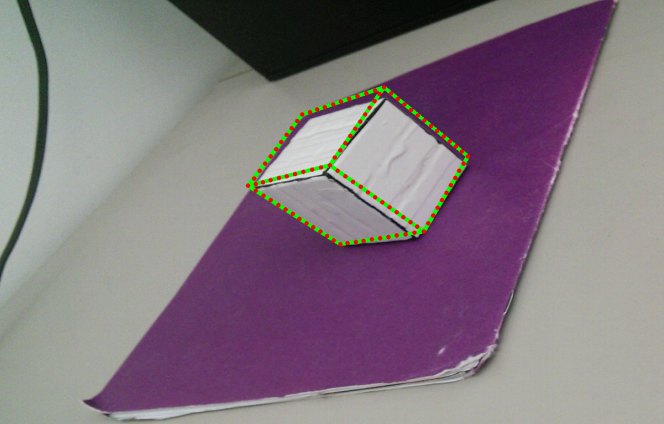
\includegraphics[scale=0.7]{wire.png}
	\caption{Kantenbasiertes rekursives Tracking, Bildquelle \cite{model_based} S.3}
\end{figure} 

Außerdem sind Ansätze wie \glqq optical flow based tracking\grqq{}, was zeitliche Informationen, entnommen aus der Bewegung der Projektion des Objekts relativ zur Bildebene verwendet, sowie texturbasierte Ansätze verbreitet. (vgl. \cite{model_based} S.1-2)



\subsection{Natürliches Feature Tracking}

Natürliches Feature Tracking ist ein bildbasiertes Verfahren und kann die Position des Gerätes zur Umgebung, ohne das Wissen über einen vorherigen Zustand, bestimmen. Diese Methode ist in der Regel sehr rechenintensiv und benötigt hohe Prozessorleistung. (vgl. \cite{model_based} S.1-2) Diese Technik verwendet die Merkmale von Objekten in der echten Welt und erkennt die natürlichen Eigenschaften dieser. Diese Merkmale werden Features genannt und sind typischerweise, basierend auf einem mathematischem Algorithmus, sehr gut unterscheidbar und außern sich in der Form von Ecken, Kanten oder starke Kontrasten. Die Feature Deskriptoren eines Bildes werden zur späteren Erkennung gespeichert. Anhand des gespeicherten Datensets aus Merkmalen kann dann erkannt werden, ob ein Bild den gleichen Inhalt zeigt, unabhängig von Entfernung, Orientierung, Beleuchtungsintensität, Rauschen oder Verdeckung. (vgl. \cite{comparative_sdks} S.13) Es gibt eine Vielzahl an natürlichen Feature Tracking und Matching Systemen, wie SIFT (Scale-Invariant Feature Transform), SURF (Speeded Up Robust Features), FAST (Features from Accelerated Segment Test), BRIEF (Binary Robust Independent Elementary Features) oder ORB (Oriented FAST and Rotated BRIEF). Diese unterscheiden sich hauptsächlich durch die erkannten Bildmerkmale im Videobild und dem erzeugtem Modell der Umgebung, die verfolgt werden soll. Die Grundsätzliche Pipeline kann wie in Abbildung 2.3 dargestellt, beschrieben werden.

\begin{figure}[H]
	\centering
	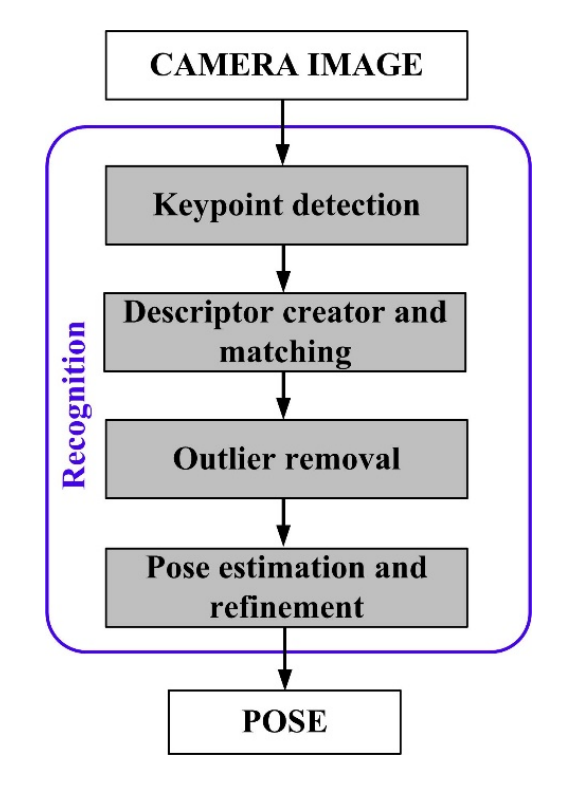
\includegraphics[scale=0.5]{tracking_pipeline.png}
	\caption{Tracking Pipeline Bildquelle \cite{natural_feature}}
\end{figure} 

Die Erstellung und das Matching der Deskriptoren hängt von der Wahl des Deskriptorssystems ab. Bei SIFT beispielsweise schätzt der Algorithmus die dominante Orientierung des Keypoints mit Hilfe von Gradienten, kompensiert die erkannte Orientierung und beschreibt abschließend die Keypoints in Bezug zu den Gradienten der Umgebung. Die erkannten Deskriptoren werden in eine Datenbank gespeichert, in welcher dann, während des Echtzeit Trackings, auf Gemeinsamkeiten geprüft werden kann.  (vgl. \cite{natural_feature} S.28-29) 


FAST hat eine ähnliche Vorgehensweise, ist jedoch um ein vielfaches schneller als SIFT. Wie in Abbildung 2.4 zu sehen ist, arbeitet der ursprüngliche Segementtest mit einem Kreis von 16 Pixeln um den Eckenkandidaten $p$. 

\begin{figure}[H]
	\centering
	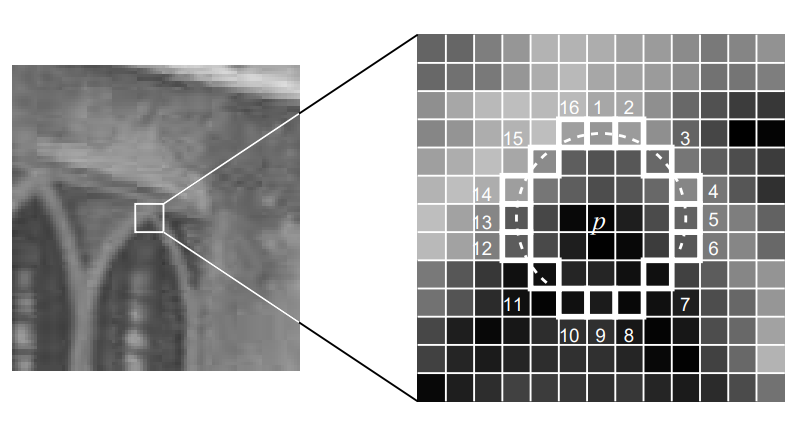
\includegraphics[scale=0.5]{fast.png}
	\caption{12 Punkt Segment Test für die Eckenerkennung \cite{fast}}
\end{figure}


Der Detektor klassifiziert $p$ als Ecke, wenn es ein Set von $n$ zusammenhängenden Pixeln im Kreis gibt, die alle heller als der Kandidat $I_p$, addiert mit einem Grenzwert $t$, oder alle dunkler als $I_p - t$ sind. $n$ ist zwölf, da dies einen High Speed Test ermöglicht, mit dem eine große Anzahl an Nicht-Ecken schnell ausgeschlossen werden kann. Der Test untersucht nur die vier Pixel 1, 5, 9 und 13. Wenn $p$ eine Ecke ist, dann müssen mindestens drei der vier Pixel heller als $I_p + t$ oder dunkler als $I_p - t$  sein. Wenn dies nicht zutrifft, ist $p$ keine Ecke. (vgl. \cite{fast} S.4-5)

\glqq Outlier removal\grqq{} oder auch die Ausreißerbeseitigung besteht aus einer Reihe von Techniken zur Entfernung von unerwünschten, falsch erkannten Keypoints, beginnend mit günstigen Methoden (einfache geometrische Tests) und abschließend mit teuren, homographie basierten Tests. (vgl. \cite{natural_feature} S.28-29) 


Die planare Homographie bezieht sich auf die dreidimensionale Lage zwischen zwei Bildebenen. Betrachtet man das erst Set and korrespondierender Punkte, $(x,y)$ im ersten Bild und $(x',y')$ im zweiten. Dann bildet die Homographie $H$ diese wie folgt ab.

\begin{equation}
  s  
  		\begin{bmatrix}
		x'\\
		y'\\
		1
     	\end{bmatrix}
     = H
     	\begin{bmatrix}
		x\\
		y\\
		1
     	\end{bmatrix}
      = 
     	\begin{bmatrix}
		h_{11} & h_{12} & h_{13}\\
		h_{21} & h_{22} & h_{23}\\
		h_{31} & h_{32} & h_{33}
     	\end{bmatrix}
      \
     	\begin{bmatrix}
		x\\
		y\\
		1
     	\end{bmatrix}
\end{equation}

Die Homographiematrix ist eine 3x3 Matrix mit 8 DoF (Degrees of Freedom). Sie wird standardmäßig normalisiert mit: 

\begin{equation}
h_33 = 1
\end{equation}

oder 
\begin{equation}
h²_{11} + h²_{12} + h²_{13} + h²_{21} + h²_{22} + h²_{23} + h²_{31} + h²_{32} + h²_{33} = 1
\end{equation}

Homographie wird in vielen Anwendungsbereichen, wie Panoramaerstellung, Bildausrichtung, perspektivischer Entzerrung oder für die Schätzung der Kameraposition in Augmented Reality verwendet. (vgl. \cite{homography}) Die Resultate der Homographie werden als Ausgangspunkt für die \glqq Pose Estimation\grqq{} (Positionsschätzung) der Kamera verwendet.  Eric Marchand et al. \cite{natural_feature} beschreiben die Positionsschätzung als Problem, welches ursprünglich in der Photogrammetrie ihren Ursprung fand und als \glqq Space Resection\grqq{} bekannt ist. Sie definieren sie folgendermaßen. \glqq given a set of correspondences between 3D
features and their projections in the images plane, pose estimation
consists in computing the position and orientation of the camera \grqq{}.

\url{http://sci-hub.tw/10.1109/TVCG.2015.2513408} !!!! <- sehr gute quelle

 Abschließend wird, basierend auf dem Gauß-Newton-Verfahren eine Reduzierung des \glqq re-projection error\grqq{} erreicht. Typischerweise sind zwei bis vier Wiederholungen genug. (vgl. \cite{natural_feature} S.28-29)

\section{Photogrammetrie vs. SLAM für Augmented Reality}

In diesem Kapitel wurde eine Einführung in Augmented Reality, deren Vorraussetzungen und aktuellen Umsetzungen dargelegt. Im folgenden Teil dieser Arbeit wird Photogrammetrie, sowie SLAM (Simultaneous Localisation and Mapping), welches von den meisten Augmented Reality SDKs inzwischen verwendet wird, beschrieben. Anschließend wird ein Vergleich der beiden Verfahren durchgeführt, um Gemeinsamkeiten, Unterschiede, sowie Möglichkeiten und Schwächen der einzelnen Verfahren aufzuzeigen und in Kontext zu bringen. Anschließend wird evaluiert ob photogrammetrische Verfahren in Kontext der Augmented Reality eingesetzt werden können.


  \chapter{Photogrammetrie}

\section{Einführung in die Photogrammetrie}

\section{Mathe in der Photogrammetrie}

\section{Pipeline}

\subsection{Feature Matching}

\subsection{Image Matching}

\subsection{Structure from Motion}

6.2 Structure from motion

\url{http://sci-hub.tw/https://doi.org/10.1007/s10462-012-9365-8}

\subsection{Depth Maps}

\section{Photogrammetrie für Smartphones}

\section{Evaluierung der photogrammetrischen Technologie für Echtzeit AR Anwendungen}
  \chapter{Verfahren zur Generierung von Mapping Daten der Umwelt}

\section{Simultaneous Localisation and Mapping}

Simultaneous Localisation and Mapping, kurz SLAM, ist das Problem der Auswertung einer unbekannten Umgebung und Erstellung einer Map, während gleichzeitig die lokale Position innerhalb dieser Map bestimmt wird. Die Lösung dieses SLAM Problems war vorallem in der Robotik eine fundamentale Aufgabe der letzten zwei Jahrzehnte. Dabei ist SLAM ein Alltagsproblem: Das Problem der räumlichen Erkundung. Jeder Mensch und jedes Tier hat dieses Verfahren gemeistert und benutzt es unterbewusst zur Navigation in unserer Realität. Die Lösung für dieses Problems, wenn es für einen Roboter automatisiert ausgeführt werden soll, ist dagegen sehr komplex. Durch das Meistern dieser Technik kann man Roboter wirklich autonom steuern. 
Bei SLAM wird die Bewegung des Objekts an sich durch den Raum und die Position aller zur positionsbestimmung notwendigen Merkmale berechnet, ohne auf vorheriges Wissen, über Position oder Lage im Raum, Kenntniss zu haben. (vgl. \cite{slam} S. 1-2) 

Dabei benötigt der Roboter mindestens einen exterozeptiven Sensor um äußere Informationen zu sammeln.
SLAM besteht aus drei grundlegenden Operationen, die iterativ pro Zeitintervall ausgeführt werden.

\textbf{Der Roboter bewegt} sich und erreicht eine neue Position in der Umwelt. Diese Bewegung erzeugt, durch unvermeidbares Rauschen und Fehler, Ungewissheit über die wirkliche Position des Roboters. Eine automatisierte Lösung benötigt ein mathematisches Modell für diese Bewegung. Dies ist das \glqq\textit{Motion Model}\grqq

\textbf{Der Roboter entdeckt neue Features} in seiner Umgebung, welche in die Umgebungskarte aufgenommen werden müssen. Diese Features heißen \glqq Landmarks\grqq . Da die Position der Landmarks, durch Fehler in den exterozeptiven Sensoren und die Position des Roboters ungewiss ist, müssen diese beiden Faktoren passend arrangiert werden. Eine automatisierte Lösung benötigt ein mathematisches Modell, das die Position der Landmarks anhand er Sensordaten bestimmt. Dies ist das \glqq textit{Inverse Oberservation Model}. \grqq

\textbf{Der Roboter entdeckt Landmarks, die schon gemappt wurden} und verwendet diese um seine eigene Position, sowie die aller Landmarks zu korrigieren. Diese Operation reduziert die Unsicherheit über den Standort des Roboters, sowie der Landmarks. Die automatisierte Lösung erfordert ein mathemathisches Modell, um die Werte der Messungen aus den prognostizierten Positionen der Landmarks und der Position des Roboters zu berechnen. Dies ist das \glqq \textit{Direct Observation Model} \grqq

Mit diesen drei Modellen ist es möglich eine automatisierte Lösung für SLAM zu entwerfen. Diese Lösung muss diese drei Modelle verbinden und alle Daten korrekt und oganisiert halten, sowie die korrekten Entscheidungen bei jedem Schritt machen. (vgl. \cite{ekf_slam} S.2-3)



\begin{figure}[H]
	\centering
	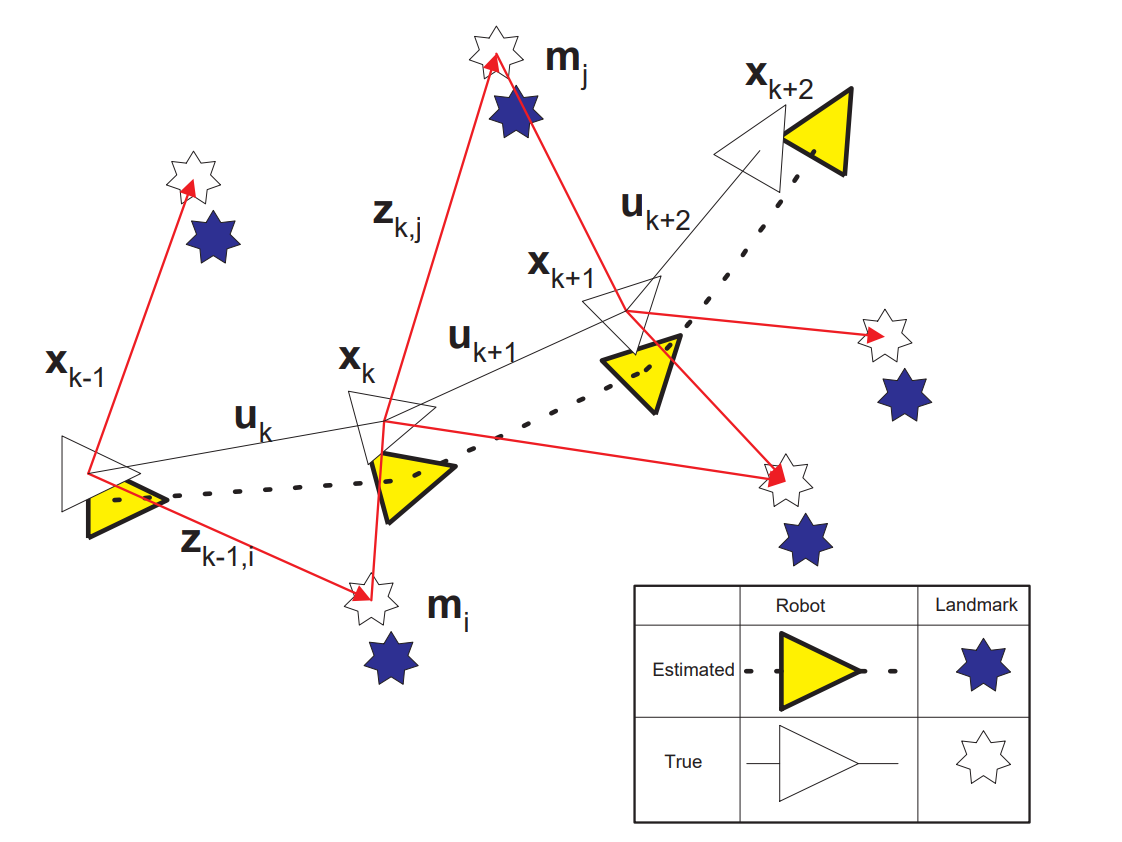
\includegraphics[scale=0.35]{slam_problem.png}
	\caption{Das SLAM Problem: Die wahren absoluten Positionen der extrahierten Features sind nie wirklich bekannt. Bildquelle \cite{slam}}
\end{figure} 

Wie in Abbildung 3.1. erkennbar ist, bewegt sich ein Roboter durch eine unbekannte Umgebung und nimmt mit seinem Sensor Features der näheren Objekte (Landmarks) auf. Wobei \large\textbf{x}\normalsize\textit{k} der Vektor des Roboters,  \large\textbf{u}\normalsize\textit{k} der Bewegungsvektor, \large\textbf{m}\normalsize\textit{i} der Vektor des Landmarks und \large\textbf{z}\normalsize\textit{ik} die Oberservation eines Landmarks durch den Roboter zur Zeit \large\textit{k }\normalsize sind. Wie man sehen kann, ist der Fehler zwischen echten und geschätzten Landmarks, bei allen geschätzten Landmarks ähnlich, was an der initialen Betrachtung der Umgebung liegt. Zu diesem Zeitpunk wird nur das erste Feature erkannt. Daraus kann man schließen, dass die Fehler in der Schätzung der Landmarkpositionen korrelieren. Praktisch bedeutet dies, dass die relative Position zweier Landmarks, \large\textbf{m}\normalsize\textit{i} - \large\textbf{m}\normalsize\textit{j} zueinander sehr genau sein kann, auch wenn die absolute Position sehr ungenau ist. 

Je mehr Landmarks in das Modell aufgenommen werden, desto gleichbleibend besser wird das Modell der relativen Positionen, egal wie sich der Roboter bewegt. Dieser Prozess wird in Abbildung 3.2. veranschaulicht.

\begin{figure}[H]
	\centering
	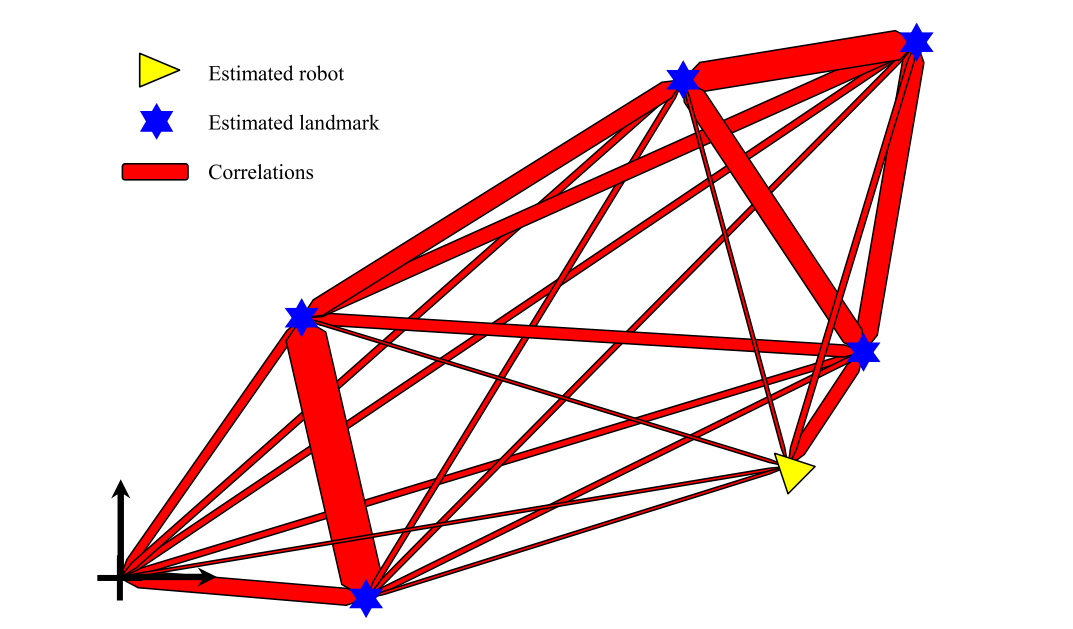
\includegraphics[scale=0.55]{slam_springs.png}
	\caption{Die Landmarks sind durch Federn verbunden, welche die Korrelation zwischen ihnen darstellen.  Bildquelle \cite{slam}}
\end{figure}  

Während sich der Roboter durch die Umgebung bewegt, werden die Korrelationen stetig aktualisiert. Je mehr Beobachtungen über die Umwelt gemacht werden, desto steifer werden die Federn in diesem Modell. Im Nachhinein werden neue Beobachtungen von Landmarks durch das ganze Netzwerk propagiert und je nach Input, kleinere oder größere Anpassungen vorgenommen.

Lösungen für das SLAM Problem benötigen eine angemessene Repräsentation für die Observierungen der Landmarks, welche eine konsistente und schnelle Berechnung ermöglichen. Die geläufigste Repräsentation besteht in der Form einer Zustandsraumdarstellung mit Gaußschen Rauschen, was zur Verwendung des \glqq Extended Kalman Filter\grqq (EKF) führt. Eine weitere alternative Repräsentation ist die Beschreibung der Features als Datenset aus Stichproben in einer nicht gaußschen Wahrscheinlichkeitsverteilung. Diese Methodik benutzt den \glqq Rao-Blackwellised particle filter\grqq oder den Fast-SLAM Algorithmus. (vgl. \cite{slam} S. 2-4)


\subsection{Extended Kalman Filter - SLAM}
Der Kalman Filter ist eine Schätzfunktion für das \glqq linear-quadratic-problem\grqq , welches das Problem der Schätzung des augenblicklichen Zustands eines linearen dynamischen Systems, gestört durch weißes Rauschen, darstellt. Der Kalman Filter wird auch dazu benutzt um die mögliche Zukunft von dynamischen Systemen vorherzusagen, die von Menschen nicht kontrolliert werden können, wie zum Beispiel die Flugbahn von Himmelskörpern, oder der Kurs von gehandelten Rohstoffen. (vgl. \cite{ekf} S.1)

Bei Extended Kalman Filter - SLAM ist die Map ein großer Stapel an Vektor und Sensordaten, sowie Zuständen von Landmarks.

\begin{equation}
  x =  \begin{bmatrix}
		R\\
		M
     	\end{bmatrix}
     = \begin{bmatrix}
		R\\
		L_1\\
		...\\
		L_n
     	\end{bmatrix}
\end{equation}

\( R\) ist der Zustand des Roboters und \( M = (L_1, ..., L_n)\)  ist das Set an Zuständen der Landmarks.
Bei EKF wird die Map durch eine gaußsche Variable modelliert, die den Mittelwert und die Kovarianzmatrix des Zustandsvektors verwendet, die jeweils durch \(\overline{x}\) und \(P\) beschrieben werden. Das Ziel ist es die Map \{\(\overline{x}, P\)\} zu allen Zeiten auf dem aktuellsten Stand zu halten.


\begin{equation}
  \overline{x} =  
  		\begin{bmatrix}
		\overline{R}\\
		\overline{M}
     	\end{bmatrix}
     = 
     	\begin{bmatrix}
		\overline{R}\\
		\overline{L_1}\\
		...\\
		\overline{L_n}
     	\end{bmatrix}
     	\quad\quad
     P = 
     	\begin{bmatrix}
		P_{RR} & P_{RM}\\
		P_{MR} & P_{MM}
     	\end{bmatrix}
     = 
     	\begin{bmatrix}
		P_{RR} & P_{RL1} & ... & P_{RLn}\\
		P_{L1R} & P_{L1L1} & ... & P_{L1Ln}\\
		... & ... & ... & ... \\
		P_{LnR} & P_{LnL1} & ... & P_{LnLn}
     	\end{bmatrix}
\end{equation}

Diese Map, die als stochastische Map bezeichnet wird, wird durch die Vorhersage- und Korrekturprozesse des EKF in Stand gehalten. Um eine echte Erkundung der Umgebung zu erreichen, wird der EKF Algorithmus mit einem extra Schritt der Landmark Erkennung und Initialisierung gestartet, bei dem neue Landmarks der Map hinzugefügt werden. Die Landmark Initialisierung erfolgt durch eine Umkehrung der Bewertungsfunktion und der Verwendung dieser und der Ableitungsmatrix, um die beobachteten Landmarks und die benötigten Co- und Crossvarianzen für den Rest der Map zu berechnen. Diese Beziehungen werden dann an den Zustandsvektor und die Kovarianzmatrix angehängt. (vgl. \cite{ekf_slam} S.6-7)


\url{http://www.iri.upc.edu/people/jsola/JoanSola/objectes/curs_SLAM/SLAM2D/SLAM%20course.pdf}

\subsection{FAST-SLAM}

\url{http://www.cs.cmu.edu/~mmde/mmdeaaai2002.pdf}
\url{http://srl.informatik.uni-freiburg.de/publicationsdir/grisettiRAS07.pdf}


\subsection{SLAM für mobiles Augumented Reality}

Das Ziel von Augumented Reality ist es virtuelle Objekte oder Informationen in die echte Welt zu integrieren, um den Benutzer zusätzliche Informationen in die betrachtete Szene zu liefern. Dazu ist es notwendig, die echte und die virtuelle Welt präzise aneinander auszurichten. Dann kann für jedes Frame aus der Sequenz des Videobildes die genaue Position des mobilen Gerätes bestimmt werden. Um dieses Ziel des exakten Matchings von Realität und generierter Virtueller Realität zu erreichen, ist "Camera Localization", also die Lokalisierung der Kamera im dreidimensionalen Raum, anhand von aufgenommenen zweidimensionalen Daten, die Schlüsseltechnologie für alle Augumented Reality Anwendungen. (vgl. \cite{slam_mobile} S.1)

\url{https://hal.inria.fr/hal-00994756/document}
\url{https://pdfs.semanticscholar.org/00f4/41387f04f40aad6491ce23bdeb0ece17d12e.pdf}



\subsection{SLAM als Core für viele AR APIs}
  \chapter{Vergleich von Photogrammetrie und SLAM}

\section{Ähnlichkeiten und Unterschiede}
Es ist inzwischen allgemein bekannt, dass Photogrammetrie und geometrische Computer Vision zwei eng zusammenhängende Disziplinen sind. Sie haben viele ähnliche Aufgabenstellungen und Ziele, wie Kalibrierung, Orientierung und Rekonstruktion. Viele Arbeiten und Forschungen beziehen sich auf beide Gebiete, wie relative Orientierung (Philip, 1996; Nistèr, 2004), die räumliche Analyse von Einzelbildern (Masry, 1981; Lepetit et al., 2009), Feature Erkennung  (Förstner \& Gülch, 1986;
Lowe, 2004) oder etwa der Bündelblockausgeleich  (Triggs et al., 2000). Dabei sollte beachtet werden, dass viele dieser Probleme erst in der Photogrammetrie untersucht und beschrieben worden sind und erst später in der Computer Vision signifikant weiter entwickelt wurden. Dies hat die Kommunikation zwischen beiden Fachbereichen gefördert. (vgl. \cite{ph_vs_cv} S.93)

\url{https://elib.uni-stuttgart.de/bitstream/11682/3934/1/Tang_Uni.pdf} 

Seite 93, Unterschiede und gemeinsamkeiten 

\section{Analyse der Echtzeitfähigkeit}


\url{https://phowo.ifp.uni-stuttgart.de/publications/phowo05/280foerstner.pdf}



  \chapter{Implementation einer AR Anwendung für Android}
Im Rahmen des Praxisteils dieser Arbeit ist eine Applikation für Android basierte Smartphones erstellt worden. In diesem Praxisteil werden die verwendeten Tools und Frameworks, um die Augmented Reality Anwendung zu erstellen, beschrieben. Das im folgenden vorgestellte Framework ARCore, implementiert den Simultaneous Location and Mapping Ansatz und ist als einzige AR-Programmierschnittstelle Open Source (Siehe Tabelle S.29).



\section{ARCore}
ARCore, das von Google entwickelt wird und das seit März 2018 verfügbar ist, ist der Nachfolger des ebenfalls von Google ins Leben gerufene Projekt Tango, welches jedoch spezielle \glqq Time-of-flight\grqq{} (TOF) Kameras benötigt, um Distanzen im Raum mithilfe des Lichtlaufzeitverfahrens zu messen. Dieser Ansatz hat sich wegen der fehlenden technischen Voraussetzungen der meisten Android Geräte nicht durchgesetzt. Da Google mit dem von Apple veröffentlichen Framework ARKit gleichziehen wollte, wurde Projekt Tango beendet und durch ARCore ersetzt. ARCore verwendet drei Schlüsselfunktionen um virtuelle Objekte in die reale Welt zu integrieren (vgl. \cite{arcore}):

\begin{itemize}
\item \textbf{Motion Tracking} ermöglicht es dem Smartphone seine Position relativ zur Umgebung zu verfolgen und zu verstehen.

\item \textbf{Environmental understanding} ermöglicht es dem Smartphone die Größe und Lage aller Arten von Oberflächen  zu erfassen, dazu zählen horizontale, vertikale oder schräge Oberflächen.

\item \textbf{Light estimation} ermöglicht die Abschätzung der aktuellen Lichtverhältnisse in der Umgebung, zur korrekten Beleuchtung und zur Erstellung von Schatten.
\end{itemize}

\subsection{Unterstütze Geräte}
Um eine gute und flüssige Erfahrung für den Endnutzer zu gewährleisten, müssen unterstützte Smartphones bestimmte Kriterien erfüllen. Dazu zählen die Qualität der verbauten Kamera, der Bewegungssensoren und der Designarchitektur. Weiterhin muss das Gerät über eine leistungsstarke CPU verfügen, die sich in das Hardware-Design integriert, um gute Leistung und effektive Echtzeitberechnung zu gewährleisten. Die Voraussetzungen um ARCore zu verwenden, werden wie folgt definiert:

\begin{itemize}
\item \textbf{Android 7.0} oder höher (Einige Modelle benötigen neuere Versionen).
\item Ein Gerät, das ursprünglich mit dem \textbf{Google Play Store} ausgeliefert wurde.
\item \textbf{Internetzugang}, um Google Play Services für AR zu installieren oder zu aktualisieren.
\end{itemize}

Aktuell werden 144 Android Smartphones, die mit dem Google Play Store ausgeliefert werden unterstützt. Weiterhin werden 29 chinesische Modelle unterstützt, bei welchen die Google Play Services manuell über die App Stores der Hersteller installiert werden müssen. Auch 20 iOS Smartphone Modelle werden unterstützt, dabei benötigt ARCore jedoch ARKit kompatible Geräte mit iOS 11.0 oder höher (Stand 22.08.2019, vgl. \cite{arcore_devices}).

\subsection{Grundlegende Konzepte}

In diesem Abschnitt werden grundlegende Funktionen, die ARCore bietet, erläutert.

\textbf{Motion Tracking} wird in ARCore mit einem Prozess namens \glqq Concurrent Odometry and Mapping\grqq{} (COM) ermöglicht. Dabei werden Features im Kamerabild erkannt und zur Bestimmung der Änderung der Position des Smartphones verwendet. Diese visuellen Informationen werden mit Trägheitsmessungen der internen Messeinheiten (IMU) des Smartphones kombiniert, um die Position und Ausrichtung der Kamera relativ zur Umwelt zu bestimmen.

Google hat sich das System und die Methodik hinter \glqq Concurrent Odometry and Mapping\grqq{} patentieren lassen. Die Beschreibung des Patents und des Systems hinter COM zeigt viele Zusammenhänge des implementierten Systems in ARCore mit SLAM und photogrammetrischen Verfahren (vgl. \cite{patent}): 

\glqq \textit{An electronic device tracks its motion in an environment while building a three-dimensional visual representation of the environment that is used to correct drift in the tracked motion. A motion tracking module estimates poses of the electronic device based on feature descriptors corresponding to the visual appearance of spatial features of objects in the environment. A mapping module builds a three-dimensional visual representation of the environment based on a stored plurality of maps, and feature descriptors and estimated device poses received from the motion tracking module. The mapping module provides the three-dimensional visual representation of the environment to a localization module, which identifies correspondences between stored and observed feature descriptors. The localization module performs a loop closure by minimizing the discrepancies between matching feature descriptors to compute a localized pose. The localized pose corrects drift in the estimated pose generated by the motion tracking module.}\grqq{}

Auch die Abbildungen über die Pipeline von COM zeigen eine hohe Übereinstimmung mit der photogrammetrischen Pipeline, sowie gegenüber SLAM, siehe Abb. 6.1.

\begin{figure}[H]
	\centering
	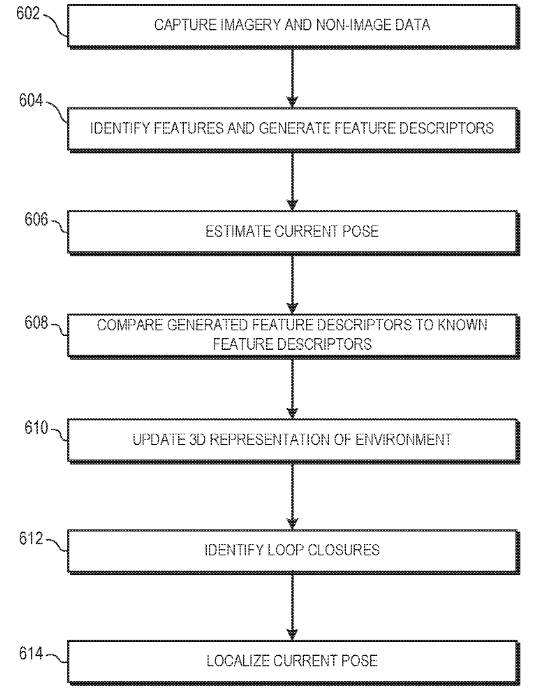
\includegraphics[scale=0.75]{com.png}
	\caption{Pipeline von COM. Bildquelle \cite{patent}}
\end{figure} 


\textbf{Environmental Understanding} wird in ARCore durch die Erkennung von Clustern von Feature Punkten auf üblichen horizontalen oder vertikalen Flächen ermöglicht. Weiterhin können die Grenzen dieser Ebenen bestimmt werden. Da ARCore zur Erkennung der Ebenen Features verwendet, werden flache oder texturlose Oberflächen, wie beispielsweise eine weiße Wand möglicherweise nicht richtig erkannt. 

\textbf{Light Estimation} wird in ARCore verwendet, um Informationen über die Beleuchtung der Umgebung zu erhalten. Dazu werden Daten wie durchschnittliche Intensität der Helligkeit oder Farbtemperatur erfasst. Anhand dieser Informationen kann mit einer Helligkeitsanpassung oder Farbkorrektur das Gefühl von Realismus in der Szene verstärkt werden, indem virtuelle Objekte unter den gleichen Bedingungen wie die echte Welt beleuchtet werden.

\textbf{User Interaction} wird in ARCore mit Hilfe von \glqq Hit-testing\grqq{} ermöglicht. Eine $(x,y)$ Koordinate auf dem Bildschirm des Smartphones wird mithilfe eines Strahls (Ray) in das Kamerabild projiziert. Alle Schnittpunkte mit Ebenen oder Merkmalspunkten des Strahls werden zusammen mit der Pose dieses Schnittpunktes zurückgegeben. Dadurch können Nutzer mit virtuellen Objekten interagieren.

\textbf{Anchors und Trackables} (Anker und trackbare Objekte) werden verwendet, da sich die Positionen von Flächen verändern kann, wenn ARCore im Lokalisierungsprozess das Verständnis für die eigene Position und das Umfeld verbessert. Um ein virtuelles Objekt zu platzieren, muss ein Anker erstellt werden, um sicherzustellen, dass ARCore die Position dieses Objekts über die Zeit verfolgt. Ebenen und Punkte sind hier eine spezielle Art von Objekt, das als \glqq Trackable\grqq{} bezeichnet wird. Virtuelle Ojekte können an bestimmten Trackables verankert werden, um sicherzustellen, dass die Beziehung zwischen virtuellen Objekt und dem zu verfolgenden Punkt oder Ebene stabil bleibt, auch wenn sich das Gerät bewegt. Das heißt, dass virtuelle Objekte, die beispielsweise auf einem gewissen Punkt am Boden platziert werden, immer noch auf exakt der gleichen Position bleiben, auch wenn die Ebene, die den Boden repräsentiert, durch ARCore angepasst und verschoben wird.

\textbf{Augmented Images} ist eine Funktion, mit der Augmented Reality Anwendungen erstellt werden können, die auf bestimmte 2D-Bilder, wie beispielsweise Produktverpackungen oder Filmposter reagieren können.

\begin{figure}[H]
	\centering
	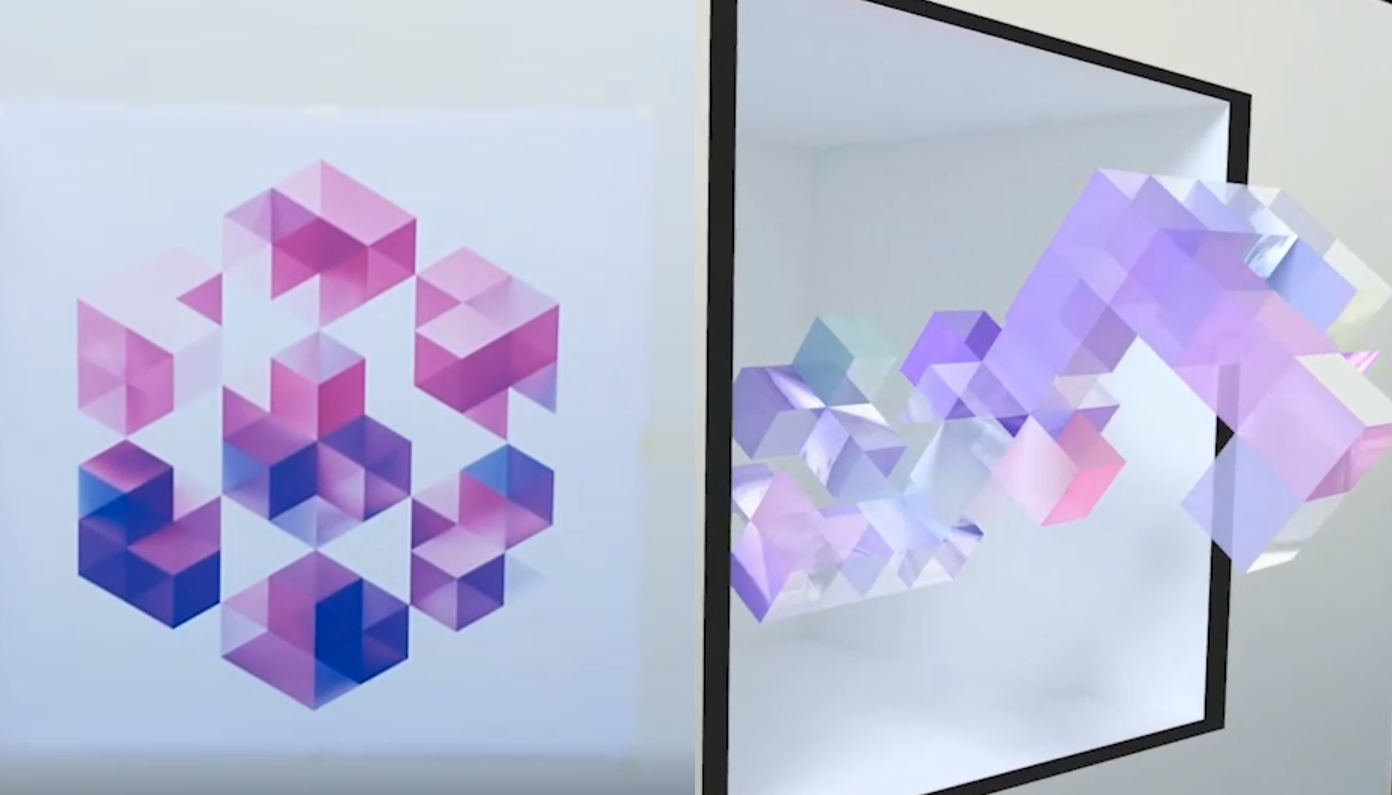
\includegraphics[scale=0.4]{augmented.png}
	\caption{Augmented Image mit ARCore, Bildquelle \cite{augmented_images}}
\end{figure} 

ARCore bietet auch eine Funktion um bewegende Bilder zu verfolgen, wie beispielsweise eine Plakatwand, auf der Seite eines fahrenden Busses. Die Bilder können offline zusammengestellt werden, um eine Bilddatenbank zu erstellen, es ist jedoch auch möglich einzelne Bilder in Echtzeit vom Gerät hinzuzufügen. Nach der Registrierung erkannt ARCore diese Bilder, sowie die Grenzen dieser und gibt eine entsprechende Pose eines virtuellen Objekts zurück.

Mithilfe der \textbf{ARCore Cloud Anchor API} können kollaborative AR Multiplayer Anwendungen erstellt werden. Dazu wird von einem Gerät der Anker und die Features der näheren Umgebung in der Cloud gespeichert. Diese Anker können dann mit anderen Benutzern auf Android- oder iOS-Geräten in der selben Umgebung geteilt werden. Mit dieser Methode können zwei Endgeräte die gleiche virtuellen 3D Objekte an exakt der gleichen Stelle im Raum rendern, so dass beide Benutzer das gleiche Erlebnis teilen (vgl. \cite{fundamental_concepts}).

\subsection{Entwicklungsumgebungen}

ARCore kann mit vielen gängigen Entwicklungsumgebungen verwendet werden. Dazu zählen Android Studio, Android Native Development Kit, Unity für Android, Unity für iOS, Unreal Engine und iOS (vgl. \cite{develop}). Im Rahmen dieser Arbeit wurde Android Studio in der Version 3.4.1, sowie ARCore in der Version 1.11.0 verwendet.

\section{Sceneform}
Sceneform ist eine Framework, das von Google entwickelt wurde und welches nahtlos in ARCore integriert werden kann. Es ermöglicht das einfache Rendern von realistischen 3D-Szenen in AR- und Nicht-AR-Anwendungen, ohne auf OpenGL zurückgreifen zu müssen. Sceneform bietet folgende Features (vgl. \cite{sceneform}):

\begin{itemize}
\item Einen high-level \textbf{Szenengraph API}.
\item Einen realistischen \textbf{physikalischen Renderer} namens \textbf{Filament}.
\item Ein \textbf{Android Studio-Plugin} zum Importieren, Anzeigen und Erstellen von \textbf{3D-Assets}.
\end{itemize}

Sceneform benötigt Android Studio Version 3.1 oder höher und wird als Plugin installiert. Es liefert ein sogenanntes \glqq ArFragment\grqq{} welches automatisch das ARCore Session Management übernimmt, sowie die notwendigen ARCore Laufzeitprüfungen durchführt. Dazu gehört die automatische Überprüfung von kompatiblen Versionen der Google Play Services für Augmented Reality und die Überprüfung der Berechtigung für Kamera und anderer Sensoren. Sind alle Überprüfungen erfolgreich, erstellt das ArFragment eine \glqq ArSceneView\grqq{} und eine ARCore Session. Mithilfe der ArSceneView kann nun das Kamerabild gerendert werden, sowie mithilfe eines \glqq PlaneRenderers\grqq{} die erkannten Ebenen zur Platzierung von virtuellen Objekten visualisert werden.

Der ArSceneView ist eine Szene zugeordnet, welche eine baumartige Datenstruktur beinhaltet. Die Nodes dieser Datenstruktur sind die zu rendernden virtuellen Objekte. Jedes Node enthält alle Informationen, um es zu rendern und damit zu interagieren. Dazu gehören Position, Ausrichtung, Modell, Kollisionsform und Event Listener. Nodes können mit anderen Nodes Eltern-Kind-Beziehungen formen, welche sich in einer baumartigen Struktur kristallisieren. Diese Struktur wird dann als Szenengraph bezeichnet. Bei jedem Einzelbild rendert Sceneform den Szenengraph aus Sicht der Kamera, welche durch das ARCore Tracking geführt wird (vgl. \cite{sceneform_google}). 

Filament ist eine physikalisch basierte Rendering (PBR) Engine für Android, die ihren Fokus auf Echtzeit Performance bei mobilen Geräten legt. Das Hauptziel von Filament sind GPUs der Klasse OpelGL ES 3.x. Die Hauptgesichtspunkte der Engine liegen in den Bereichen Qualität, Benutzerfreundlichkeit, Vertrautheit, Flexibilität und in der Größe der bereitgestellten Renderbibliothek. Physikalisch basiertes Rendering ist ein Verfahren, das eine genauere Darstellung von Materialien und deren Wechselwirkungen mit Licht im Vergleich zu herkömmlichen Echtzeitmodellen ermöglicht. Die Trennung von Materialien und Beleuchtung im Kern der PBR Methode macht es einfacher, realistische Objekte zu erstellen, die unter allen Lichtverhältnissen präsize aussehen (vgl \cite{filament}).


\section{Google Places API}

Im Rahmen dieser Arbeit wird die Google Places API, zur Abfrage von Informationen mithilfe des aktuellen Standort des Smartphones, verwendet. Die Places-API ist ein Dienst, der Informationen über bestimmte Orte mit HTTP-Anfragen zurückgibt. Places sind innerhalb der API definiert als Einrichtungen, geografische Standorte oder berühmte Points of Interest. Die Informationen die mit der API abgefragt werden können, sind etwa einfache Listen der näheren Orte, Details über die Orte in der Nähe oder Fotos der näheren Orte, aus der Google Datenbank. Die API ermöglicht auch die  Autovervöllständigung von Suchanfragen bestimmter Orte oder Querys. Jeder dieser Dienste wird als HTTP-Request aufgerufen und gibt entweder XML- oder JSON-Dateien als Antwort zurück. Alle Anfragen müssen das HTTPS Protkoll verwenden und benötigen einen eigenen API Schlüssel (vgl. \cite{places_api}).

Bei der Implementation der App wurde die \glqq Place Search\grqq{} Funktion der API verwendet. Ein Call schaut wie folgt aus:

\begin{lstlisting}[basicstyle=\small]
https://maps.googleapis.com/maps/api/place/nearbysearch/json?location=
 + LAT_LNG + &rankby=distance&keyword= + KEY_WORD + &key= + API_KEY;
\end{lstlisting}

Das Ergebnis dieses Anfrage Querys erhält eine Vielzahl an Informationen, die anschließend weiter verarbeitet werden können.





\section{Dexter}

\section{Volley}

\section{Implementierung}




  \chapter{Zusammenfassung}


Fortschritte in der Photogrammetrie sind viel zu sehr mit den Fortschritten der Computer Vision verflochten, als dass sich die Konvergenz der beiden Disziplinen umkehren wird. Photogrammetrie und Computer Vision haben die Extraktion und Rekonstruktion von Daten aus Bildmaterial zu unterschiedlichen Zeiten und mit unterschiedlichen Zielen begonnen. Als sich dann 3D-Modelle als Referenzziel herausstellten, wurde der Austausch von Ansätzen und Techniken zwischen den Disziplinen vorangetrieben (vgl. \cite{state_of_art} S.9). Dies hat dazu geführt, dass Photogrammetrie und Computer Vision verfahrenstechnisch kaum mehr unterscheidbar sind, auch wenn die ursprünglichen Anwendungsgebiete verschieden sind. 

Im Rahmen dieser Arbeit wurden Algorithmen und Konzepte aus der Photogrammetrie und der Computer Vision beschrieben und verglichen. Anschließend wurde ein Überblick über die Ziele, Unterschiede und Gemeinsamkeiten von Photogrammetrie, SLAM und SfM gegeben. Es hat sich gezeigt, dass sich diese Verfahren inhaltlich stark überschneiden, auch wenn die Fachrichtung, der historische Kontext und die Ziele von Photogrammetrie und SLAM grundverschieden sind. 

Im Praxisteil wurde eine Applikation erstellt, welche ARCore verwendet. ARCore implementiert SLAM und verwendet damit auch photogrammetrische Verfahren. Photogrammetrie kann also in Augmented Reality Anwendungen verwendet werden, auch wenn dann die Bezeichnung irreführend ist. SLAM könnte man als Echtzeit-Photogrammetrie bezeichnen, welche nicht auf größtmögliche Genauigkeit, sondern auf Schnelligkeit und Stabilität ausgelegt ist. In Zukunft wird sich die Konvergenz der in dieser Arbeit beschrieben Disziplinen noch verstärken, die Kategorisierung in die verschiedenen Fachbereiche ist jedoch, mit Sicht auf die Anwendungsgebiete, Philosophien und den historischen Ursprung, sinnvoll.

Vielen Dank an Prof. Dr. Tobias Lenz und Prof. Dr. Klaus Jung die Betreuung und Korrektur dieser Arbeit.
	

  % ... weitere Kapitel
 
  % Literaturverzeichnis
  \phantomsection
  \addcontentsline{toc}{chapter}{Literaturverzeichnis}
  \begin{thebibliography}{10}
  
  
    \bibitem[1]{photo} Heipke, C. (2017), \glqq Photogrammetrie und Fernerkundung \grqq, 1.Auflage, Berlin: Springer Verlag, S. 5-7.
    
    \bibitem[2]{slam} Hugh Durrant-Whyte, Tim Bailey (2006), Simultaneous Localisation and Mapping (SLAM): Part I The Essential Algorithms. URL: \url{https://people.eecs.berkeley.edu/~pabbeel/cs287-fa09/readings/Durrant-Whyte_Bailey_SLAM-tutorial-I.pdf} (Zuletzt abgerufen am 09.07.2019)
    

	\bibitem[3]{slam_mobile} P. Martin, E. Marchand, P. Houlier, I. Marchal. Mapping and re-localization for mobile augmented reality. IEEE Int. Conf. on Image Processing, Oct 2014, Paris, France.
URL: \url{https://hal.inria.fr/hal-00994756/document} (Zuletzt abgerufen am 09.07.2019) 

	\bibitem[4]{ekf_slam} Joan Sol`a, (2014), Simulataneous localization and mapping with the extended Kalman filter. URL: \url{http://www.iri.upc.edu/people/jsola/JoanSola/objectes/curs_SLAM/SLAM2D/SLAM\%20course.pdf} (Zuletzt aufgerufen am 10.07.2019)
    
    \bibitem[5]{ekf} Mohinder S. Grewal, Angus P. Andrews (2001), Kalman Filtering: Theory and Practice with MATLAB. URL: \url{http://staff.ulsu.ru/semoushin/_index/_pilocus/_gist/docs/mycourseware/13-stochmod/2-reading/grewal.pdf} (Zuletzt aufgerufen am 10.07.2019)

	\bibitem[6]{ekf_problems} M. Montemerlo, S. Thrun, D. Koller, B. Wegbreit (2002). FastSLAM: A Factored Solution to the Simultaneous Localization and Mapping Problem. URL: \url{http://robots.stanford.edu/papers/montemerlo.fastslam-tr.pdf} (Zuletzt aufgerufen am 11.07.2019) 
	
	\bibitem[7]{rao} G. Grisetti, G.D. Tipaldi, C. Stachniss, W. Burgard, D. Nardi (2007). Fast and accurate SLAM with Rao-Blackwellized particle filters. URL: \url{http://srl.informatik.uni-freiburg.de/publicationsdir/grisettiRAS07.pdf} (Zuletzt aufgerufen am 11.07.2019)

\bibitem[8]{slam_studi} M. Mengelkoch (2007). Implementieren des FastSLAM Algorithmus zur
Kartenerstellung in Echtzeit. URL: \url{https://kola.opus.hbz-nrw.de/opus45-kola/frontdoor/deliver/index/docId/183/file/sa-00.pdf} (Zuletzt aufgerufen am 11.07.2019)

\bibitem[9]{survey} J. Fuentes-Pacheco, J. Ruiz-Ascencio, J.M. Rendón-Mancha (2012). Visual simultaneous localization and mapping: a survey. In: J.M. Artif Intell Rev (2015) 43: 55. Springer Netherlands. DOI: \url{https://doi.org/10.1007/s10462-012-9365-8}

\bibitem[10]{ar_slam} J. Halvarsson, (2018), Using SLAM-based technology to improve directional navigation in an Augmented Reality game. URL: \url{http://umu.diva-portal.org/smash/get/diva2:1245293/FULLTEXT01.pdf} (Zuletzt aufgerufen am 11.07.2019)

\bibitem[11]{ar_vr} P. Milgram, H. Takemura, A. Utsumi, F. Kishino (1994), Augmented Reality: A class of displays on the reality-virtuality continuum. URL: \url{http://etclab.mie.utoronto.ca/publication/1994/Milgram_Takemura_SPIE1994.pdf} (Zuletzt aufgerufen am 16.07.2019)

\bibitem[12]{sdks} A. Hanafi, L. Elaachak, M. Bouhorma (2019), A comparative Study of Augmented Reality SDKs to Develop an Educational Application in Chemical Field. DOI: 10.1145/3320326.3320386

\bibitem[13]{comparative_sdks} D. Amin, S. Govilkar (2015), Comparative Study of Augmented Reality
SDK’s. International Journal on Computational Sciences \& Applications (IJCSA) Vol.5, No.1, February 2015 URL: \url{https://pdfs.semanticscholar.org/e752/17e8897cb46b466d6ba83e909cca4ecff8f2.pdf} (Zuletzt aufgerufen am 16.07.2019)

\bibitem[14]{model_based} M. Lowney, A. S. Raj (2016), Model Based Tracking for Augmented Reality
on Mobile Devices. URL: \url{https://web.stanford.edu/class/ee368/Project_Autumn_1617/Reports/report_lowney_raj.pdf} (Zuletzt aufgerufen am 16.07.2019)

\bibitem[15]{natural_feature} S. Ćuković, M. Gattullo, F. Pankratz, G. Devedzic, E. Carrabba, K. Baizid (2015), Marker Based vs. Natural Feature Tracking Augmented Reality Visualization of the 3D Foot Phantom. URL: \url{https://www.researchgate.net/publication/278668320_Marker_Based_vs_Natural_Feature_Tracking_Augmented_Reality_Visualization_of_the_3D_Foot_Phantom} (Zuletzt aufgerufen am 17.07.2019)

\bibitem[16]{homography} Basic concepts of the homography explained with code. URL: \url{https://docs.opencv.org/3.4.1/d9/dab/tutorial_homography.html} (Zuletzt aufgerufen am 17.07.2019)

\bibitem[17]{camera_pose} M. Maidi, J.Y. Didier, F. Ababsa, M. Mallem (2008), A performance study for camera pose estimation using visual marker based tracking. URL: \url{https://www.academia.edu/13152554/A_performance_study_for_camera_pose_estimation_using_visual_marker_based_tracking}
(Zuletzt aufgerufen am 18.07.2019)

\bibitem[18]{vorraussetzungen} A. Pinz, M. Brandner, H. Ganster, A. Kusej, P. Lang, M. Ribo (2002) Hybrid Tracking for Augmented Reality. URL: \url{https://www.researchgate.net/publication/229025765_Hybrid_tracking_for_augmented_reality} (Zuletzt aufgerufen am 18.07.2019)

\bibitem[19]{fast} E. Rosten, T. Drummond (2006) Machine learning for high-speed corner detection. URL: \url{https://www.edwardrosten.com/work/rosten_2006_machine.pdf} (Zuletzt aufgerufen am 18.07.2019)

\bibitem[20]{fiundations_pg} K. Schindler (2014) Mathematical Foundations of
Photogrammetry. URL: \url{https://ethz.ch/content/dam/ethz/special-interest/baug/igp/photogrammetry-remote-sensing-dam/documents/pdf/math-of-photogrammetry.pdf} (Zuletzt aufgerufen am 19.07.2019)

\bibitem[21]{pp} A.S. Alturki, J.S. Loomias (2016) Camera Principal Point Estimation from Vanishing Points. DOI: 10.1109/NAECON.2016.7856820 (Zuletzt aufgerufen am 19.07.2019)

\bibitem[22]{exterior_review} P. Grussenmeyer, O. Al Khalil (2002) Solutions for Exterior Orientation in Photogrammetry: A Review. Photogrammetric Record, 17(100):615-634. URL: \url{https://hal.archives-ouvertes.fr/hal-00276983/document} (Zuletzt aufgerufen am 19.07.2019)

\bibitem[23]{comparative_conditions_study} K.L.A. El-Ashmawy (2015). A comparison study between collinearity condition, coplanarity condition, and direct linear transformation (DLT) method for camera exterior orientation parameters determination. Geodesy and Cartography, 41(2), 66–73. URL:\url{https://journals.vgtu.lt/index.php/GAC/article/view/2837/2334} (Zuletzt aufgerufen am 19.07.2019)

\bibitem[24]{coll_exterior} E.E. Elnima (2015) A solution for exterior and relative orientation
in photogrammetry, a genetic evolution approach. Journal of King Saud University – Engineering Sciences. URL: \url{https://core.ac.uk/download/pdf/82822280.pdf}  (Zuletzt aufgerufen am 22.07.2019)

\bibitem[25]{lev_efficient} M. Lourakis, A. Argyros (2005) Is Levenberg-Marquardt the Most Efficient Optimization Algorithm for Implementing Bundle Adjustment? URL: \url{https://www.ics.forth.gr/_publications/0201-P0401-lourakis-levenberg.pdf} (Zuletzt aufgerufen am 20.08.2019) 

\bibitem[26]{state_of_art} G. Forlani, R. Roncella, C. Nardinocchi (2015) Where is photogrammetry heading to? State of the art and trends. Rendiconti Lincei, 26(S1), 85–96. DOI:10.1007/s12210-015-0381-x  (Zuletzt aufgerufen am 24.07.2019)

\bibitem[27]{dlt} K. L. El-Ashmawy (2018) Using direct linear Transformation (DLT) Method for
aerial Photogrammetry Applications. Geodesy and Cartography 2018 Volume 44 Issue 3: 71–79. URL: \url{https://journals.vgtu.lt/index.php/GAC/article/download/1629/5048} (Zuletzt aufgerufen am 24.07.2019)

\bibitem[28]{nonlinear_1} L. Vandenberge (2018) 13. Nonlinear least squares. URL: \url{http://www.seas.ucla.edu/~vandenbe/133A/lectures/nlls.pdf} (Zuletzt aufgerufen am 20.08.2019)

\bibitem[29]{least_quares} A. W. Gruen (1985) Adaptive least Squares Correlations:
A powerful Image Matching Technique. URL: \url{https://www.researchgate.net/publication/265292615_Adaptive_Least_Squares_Correlation_A_powerful_image_matching_technique}  (Zuletzt aufgerufen am 24.07.2019)

\bibitem[30]{nonlinear_2} S. Boyd (2016) Nonlinear Least Squares. URL: \url{https://stanford.edu/class/ee103/lectures/nlls_slides.pdf} (Zuletzt aufgerufen am 24.07.2019)

\bibitem[31]{approx_gn} S. Gratton, A. S. Lawless, N. K. Nichols (2007) Approximate Gauss–Newton Methods for Nonlinear Least Squares Problems. URL: \url{https://www.researchgate.net/publication/220133629_Approximate_Gauss-Newton_Methods_for_Nonlinear_Least_Squares_Problems} (Zuletzt aufgerufen am 30.07.2019)

\bibitem[32]{lev_mar} H. P. Gavin (2019) The Levenberg-Marquardt algorithm for
nonlinear least squares curve-fitting problems. URL: \url{http://people.duke.edu/~hpgavin/ce281/lm.pdf} (Zuletzt aufgerufen am 30.07.2019)

\bibitem[33]{levenberg} K. Levenberg (1944) A method for the solution of certain non-linear problems in least squares. URL: \url{https://www.ams.org/journals/qam/1944-02-02/S0033-569X-1944-10666-0/} (Zuletzt aufgerufen am 30.07.2019)

\bibitem[34]{bundle_adjustment} N. Börlin, P. Grussenmeyer (2013) Bundle Adjustment With and Without Damping. The Photogrammetric Record, 28(144), 396–415. DOI: 10.1111/phor.12037 (Zuletzt aufgerufen am 07.08.2019)

\bibitem[35]{robust_feature} A. Abbas, S. Ghuffar (2018) Robust Feature Matching in terrestrial Image Sequences. The International Archives of the Photogrammetry, Remote Sensing and Spatial Information Sciences, Volume XLII-3, URL: \url{https://www.researchgate.net/publication/324855190_ROBUST_FEATURE_MATCHING_IN_TERRESTRIAL_IMAGE_SEQUENCES} (Zuletzt aufgerufen am 07.08.2019)

\bibitem[36]{det_des} F. Remondino (2006) Detectors and descriptors for photogrammetric applications. URL: \url{http://3dom.fbk.eu/sites/3dom.fbk.eu/files/pdf/remondino_ISPRS_III_06.pdf} (Zuletzt aufgerufen am 07.08.2019)

\bibitem[37]{old_new_feature} A. Lingua, D. Marenchio, F. Nex (2009) A comparison between “old and new” feature extraction and matching techniques in Photogrammetry. URL: \url{https://pdfs.semanticscholar.org/b9c3/067b6fc111e1cc02f42357d5fb459a642152.pdf} (Zuletzt aufgerufen am 07.08.2019)

\bibitem[38]{efficient_bundle} Z. Qu (2018) Efficient Optimization for
Robust Bundle Adjustment. URL: \url{https://vision.in.tum.de/_media/members/demmeln/qu2018msc.pdf}  (Zuletzt aufgerufen am 08.08.2019)

\bibitem[39]{loop_closure} A. Bokovoy, K. Yakovlev (2017) Original Loop-Closure Detection Algorithm for Monocular vSLAM. Analysis of Images, Social Networks and Texts, 210–220. URL: \url{https://arxiv.org/pdf/1707.04771.pdf} (Zuletzt aufgerufen am 08.08.2019)

\bibitem[40]{orb_slam} M. Andersson, M. Baerveldt (2018) Simultaneous localization and mapping
for cars using ORB2-SLAM. URL: \url{http://publications.lib.chalmers.se/records/fulltext/256291/256291.pdf} (Zuletzt aufgerufen am 08.08.2019)

\bibitem[41]{orbslam_og}  R. Mur-Artal, J. M. M, Montiel (2015) ORB-SLAM: a Versatile and Accurate Monocular SLAM System. URL: \url{https://arxiv.org/pdf/1502.00956.pdf}(Zuletzt aufgerufen am 08.08.2019)

\bibitem[42]{brief} M. Calonder, V. Lepetit, C. Strecha, P. Fua (2010) BRIEF: Binary Robust Independent Elementary Features. URL: \url{https://www.researchgate.net/publication/221304115_BRIEF_Binary_Robust_Independent_Elementary_Features} (Zuletzt aufgerufen am 08.08.2019)

\bibitem[43]{ph_vs_cv} R. Tang (2013) Mathematical Methods for Camera Self-Calibration
in Photogrammetry and Computer Vision. URL: \url{https://elib.uni-stuttgart.de/bitstream/11682/3934/1/Tang_Uni.pdf} (Zuletzt aufgerufen am 12.08.2019)

\bibitem[44]{sfm} S. N. Sinha1, D. Steedly, R. Szeliski1 (2016) A multi-stage linear approach to structure from motion. URL: \url{https://www.microsoft.com/en-us/research/wp-content/uploads/2016/07/sinhaRMLE10_linearSfm.pdf} (Zuletzt aufgerufen am 13.08.2019)

\bibitem[45]{sfm_photo} M. J. Westobya, J. Brasington, N. F. Glasser, M. J. Hambrey, J. M. Reynolds (2012) 'Structure-from-Motion' photogrammetry: A low-cost, effective tool for geoscience applications. URL: \url{https://www.sciencedirect.com/science/article/pii/S0169555X12004217} (Zuletzt aufgerufen am 13.08.2019)

\bibitem[46]{vergleich_fraser} C. Fraser (2018) SLAM, SFM AND PHOTOGRAMMETRY: WHAT’S IN A NAME? URL: \url{https://www.isprs.org/tc2-symposium2018/images/ISPRS-Interview-Fraser.pdf} (Zuletzt aufgerufen am 13.08.2019)

\bibitem[47]{pose} F. Herranz, K. Muthukrishnan, K. Langendoen (2011) Camera pose estimation using particle filters. URL: \url{https://www.researchgate.net/publication/229033775_Camera_pose_estimation_using_particle_filters} (Zuletzt aufgerufen am 19.08.2019)

\bibitem[48]{markers} H. Le, M. Nguyen, H. Tran, W. Yeap (2017) Pictorial AR Tag with Hidden Multi-Level Bar-Code and Its Potential Applications. URL: \url{https://www.mdpi.com/2414-4088/1/3/20} (Zuletzt aufgerufen am 19.08.2019)

\bibitem[49]{sift} D. G. Lowe (1999) Object Recognition from Local Scale-Invariant Features. URL: \url{https://www.cs.ubc.ca/~lowe/papers/iccv99.pdf} (Zuletzt aufgerufen am 19.08.2019)

\bibitem[50]{pose_estimation} E. Marchand, H. Uchiyama, F. Spindler (2016) Pose Estimation for Augmented Reality: A Hands-On Survey. IEEE Transactions on Visualization and Computer Graphics, Institute of Electrical and Electronics Engineers, 2016, 22 (12), pp.2633 - 2651. URL: \url{https://hal.inria.fr/hal-01246370/document} (Zuletzt aufgerufen am 19.08.2019)

\bibitem[51]{arcore} ARCore overview. URL: \url{https://developers.google.com/ar/discover} (Zuletzt aufgerufen am 29.08.2019)

\bibitem[52]{arcore_devices} ARCore Supported Devices. URL: \url{https://developers.google.com/ar/discover/supported-devices} (Zuletzt aufgerufen am 29.08.2019)

\bibitem[53]{augmented_images} ARCore Augmented Images URL: \url{https://developers.google.com/ar/develop/java/augmented-images/} (Zuletzt aufgerufen am 29.08.2019)

\bibitem[54]{fundamental_concepts} ARCore Fundamental Concepts. URL: \url{https://developers.google.com/ar/discover/concepts} (Zuletzt aufgerufen am 29.08.2019)

\bibitem[55]{develop} ARCore Development Environment. URL: \url{https://developers.google.com/ar/develop} (Zuletzt aufgerufen am 29.08.2019)

\bibitem[56]{patent} Patent: System and method for concurrent odometry and mapping. URL: \url{https://patents.google.com/patent/US20170336511A1/en} (Zuletzt aufgerufen am 30.08.2019)

\bibitem[57]{sceneform} Sceneform SDK for Android. URL: \url{https://github.com/google-ar/sceneform-android-sdk} (Zuletzt aufgerufen am 30.08.2019)

\bibitem[58]{sceneform_google} Sceneform Overview. URL: \url{https://developers.google.com/ar/develop/java/sceneform} (Zuletzt aufgerufen am 30.08.2019)

\bibitem[59]{filament} Physically Based Rendering in Filament. URL: \url{https://google.github.io/filament/Filament.html#overview/principles} (Zuletzt aufgerufen am 30.08.2019)

\bibitem[60]{places_api} Google Places API. URL: \url{https://developers.google.com/places/web-service/intro} (Zuletzt aufgerufen am 30.08.2019)

\bibitem[61]{odometrie} Navigation mobiler Systeme. URL: \url{http://ots.fh-brandenburg.de/downloads/scripte/ams/2014-Navigation-Teil\%201.pdf} (Zuletzt aufgerufen am 02.09.2019)

\bibitem[62]{dexter} Github, Dexter: Android library that simplifies the process of requesting permissions at runtime. URL: \url{https://github.com/Karumi/Dexter} (Zuletzt aufgerufen am 02.09.2019)

\bibitem[63]{marshmallow} Android 6.0 Marshmallow. URL: \url{https://android.googleblog.com/2015/10/get-ready-for-sweet-taste-of-android-60.html}  (Zuletzt aufgerufen am 02.09.2019)

\bibitem[64]{volley} Github, Volley. URL: \url{https://github.com/google/volley} (Zuletzt aufgerufen am 03.09.2019)

\bibitem[65]{volley_ref} Volley overview. URL: \url{https://developer.android.com/training/volley/index.html} (Zuletzt aufgerufen am 03.09.2019)

\bibitem[67]{arcore_geo} Feature Request: Provide a geo-oriented world coordinate space. URL: \url{https://github.com/google-ar/arcore-android-sdk/issues/119} (Zuletzt aufgerufen am 03.09.2019)

\bibitem[68]{orbslam2} R. Mur-Artal, J. D. Tardós (2017) ORB-SLAM2: an Open-Source SLAM System for Monocular, Stereo and RGB-D Cameras. URL: \url{https://arxiv.org/pdf/1610.06475.pdf} (Zuletzt aufgerufen am 03.09.2019)










	\end{thebibliography}  
  \newpage
  
  % Anhang
  \phantomsection
  \addcontentsline{toc}{chapter}{Abbildungsverzeichnis}
  \listoffigures
  \newpage
 
  
  %\include{anhang}
\end{document}    